\documentclass[11pt,a4paper]{article}
\usepackage[utf8]{inputenc}
\usepackage[T1]{fontenc}
\usepackage{subcaption}

\usepackage[table,xcdraw]{xcolor}
\usepackage{setspace,fullpage,graphicx,mathptmx, amsmath,amssymb,amsfonts,setspace,fullpage,booktabs}
\usepackage[bookmarksnumbered=true]{hyperref} 
\hypersetup{colorlinks = true,linkcolor = blue,anchorcolor = blue,citecolor = blue,filecolor = blue,urlcolor = blue}
\usepackage[round]{natbib}
\bibliographystyle{plainnat}
\title{Mining Unstructured Clinical Notes for Mortality Prediction}
\author{Vineet Kumar (19BM6JP46) \\Rohit Bajpai (19BM6JP56)}
\begin{document}
	\maketitle
\onehalfspacing
\begin{abstract}
\noindent	Unstructured clinical data such as nursing notes
	are very less used to build a predictive model for
	post-discharge mortality despite containing rich
	information. Our work examines a simple bag of
	words model approach for 7/30/180/365 day mortality prediction. We also explored syntactic sentiment dimensions from these nursing notes as
	a predictor of mortality, and report preliminary
	survival analysis results too. Our simple BOW model
	using XGBoost achieved 0.92 AUC for 30-day
	mortality.
\end{abstract}


\section{Introduction}
Wider adoption of Electronic Health Records (EHRs) in the hospital setting has given rise to a plethora of clinical data. EHR records patient demographic details, past medical history, periodic clinical measurements like patient vitals, test reports, medical interventions, and detailed clinical/nursing notes. Structured clinical (tabular) data contain a rich but incomplete picture of the patient. Clinical notes are recorded by attending nurses in free form textual format. They contain rich information relevant to the patient's response to treatment and illness trajectory as well. To better understand high-risk patients, health systems must leverage text analytics,to derive insights from
free form clinical texts. NLP helps in interpretation of textual
data. It can aid in information extraction, conversion of unstructured to structured data, Document
categorization etc.However, due to their high free form nature utilizing these unstructured clinical descriptions (UCDs) in building clinical decision support systems is not much explored. Predicting post-discharge mortality is one of the major
research areas in health-informatics \cite{metersky2012predictors}.

\subsection{Related Works}

Recent advances in NLP and data mining has made it possible
to mine these unstructured nursing notes for mortality prediction. Hence, there has been multiple studies in model enrichment \cite{staff2013can}, patient phenotyping \cite{gehrmann2017comparing}, readmission prediction \cite{shin2019multimodal} etc.

Moreover, the latest advances in deep learning technologies (DL) have encouraged the use of deep nets in the clinical domain as well, ranging from computer-aided diagnosis to genome sequencing \cite{miotto2018deep}. Classical ML \& statistical techniques require feature engineering, which is sometimes very time consuming and requires domain expertise. In such scenarios, the DL approach has become very useful; however, due to their black-box nature, the use of these sophisticated approach is still not much appreciated in clinical decision support systems (DSSs). 


In this work, we study the post-discharge mortality prediction of patients by deriving insights from the unstructured clinical descriptions (UCDs).  The study by \citet{churpek2016multicenter} concluded that in clinical practice, simpler models are most
commonly deployed, which are easy to interpret by physicians as well as regulators.  Hence, our work will be focused on building simple as well as interpretable models which can be used for building clinical decision support tools that flag at-risk patients.

The  key contribution of our work is we have built a simple BOW model for 7/30/180/365 day mortality prediction just based on clinical notes. The performance thus achieved (0.92 AUC for 30 day mortality)  is good given its simplicity. We also explored inbuilt library based syntactic sentiment analysis for doing preliminary survival analysis.

The rest of our
paper is organised as follows --- Section: \ref{method} describes the
dataset used, patient cohort selection and routine data preprocessing methodology. Section: \ref{model} describes various models used in the experiment. Finally, Section: \ref{evaluation} presents
the evaluation metric we have chosen, their interpretation and discussions around it. 
\section{Methodology \& Dataset}\label{method}

\subsection{Dataset} We used MIMIC-III v1.4 \cite{johnson2016mimic}, which is publicly available de-identified health-related data associated with over 40,000 patients who stayed in critical care units of the Beth Israel Deaconess Medical Center between 2001 and 2012. The dataset contains information on patient demographics, vital sign measurements, lab test results, clinical procedures, medications, caregiver notes, imaging reports, and mortality labels. 

\subsection{Patient Cohort Selection}

We retrieved set of adult patients ($\geq 18$ years) with at least one associated
note from the MIMIC-III database. We specifically extracted \texttt{Nursing Progress Note} from the dataset. Check the Figure \ref{data} to understand number of notes for each category in whole dataset, we chose Nursing as it is more useful for our purpose as well as it has most number of records. 
\begin{figure}[h!]
	\centering
		\centering
		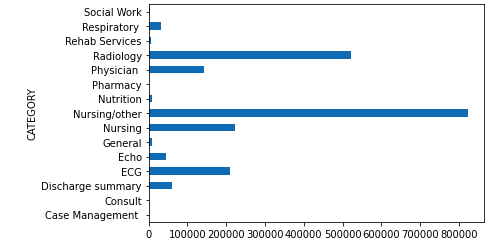
\includegraphics[width=0.55\textwidth]{notes.png}
			\caption{Numbers of Notes Per Category}
	\label{data}
\end{figure}

\subsection{Data Preparation}
We used google bigquery and its SQL dialect for our patient cohort selection. The mean number of notes per hospital admission is 32 (median: 15). We concatenated all notes of a particular patient with the same hospital admission id. A such concatenated sample note is shown in Figure  \ref{fig:note}.
\begin{figure*}[h!]
	\label{note.pdf}
	\centering
	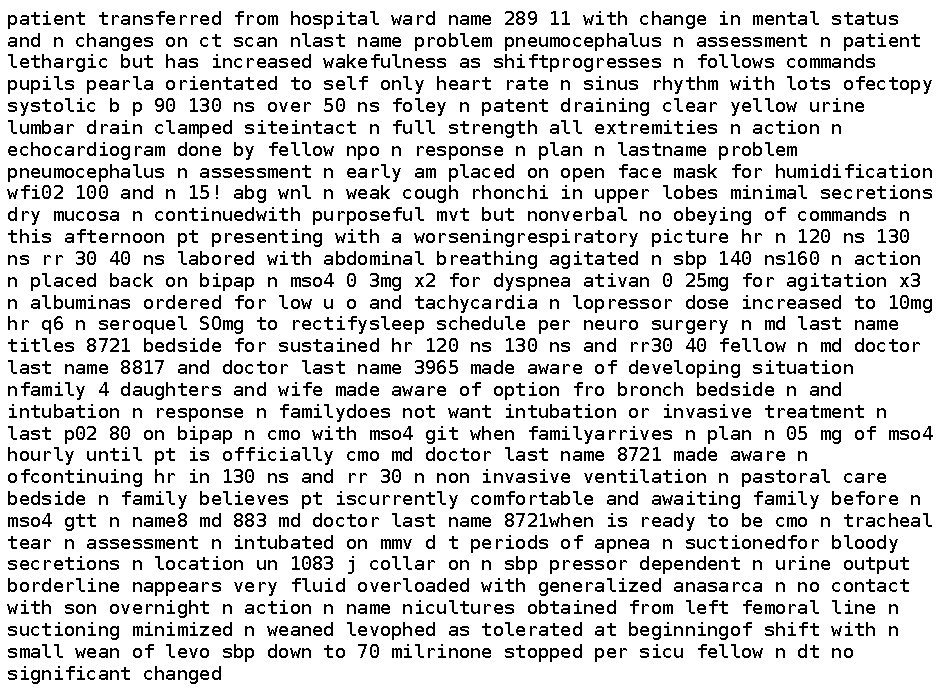
\includegraphics[width=0.84\linewidth]{note.pdf}
	\caption{Sample Concatenated Note}
	\label{fig:note}
\end{figure*}

We also created an attribute `surv\_day', which is essentially the number of days the patient has survived after discharge from the hospital. For patients whose clinical file didn't have a death date (i.e., those who are still alive) were marked as NaN. We used this `surv\_day' attribute to build some new binary labels --- `one week mortality' (if surv\_day $<$7 then 1 else 0), `thirty day mortality', `one eighty mortality', and finally a `one year mortality' label. 

\begin{table}[h!]
	\begin{center}
\begin{tabular}{lc}
	\hline
	\textbf{Attribute Label} & \textbf{Frequency (Prevalence)} \\
	\hline
	one\_week\_mortality	& 258 \\
	thirty\_day\_mortality	& 736 \\
	one\_eighty\_mortality	& 253  \\
	one\_year\_mortality	& 653 \\
	\hline %\caption{Frequency of True Labels each class}
\end{tabular}\end{center}
\caption{Prevalence in Survival Class}
\end{table}

Patients were randomly split into train (70\%), validation (15\%),
and test (15\%) sets. Since we have a limited number of True labels for any class, for example, consider thirty\_day\_mortality has train prevalence (Number of True in mortality label)  is 11\%. It has a class imbalance, to deal we this we did a minority class oversampling. 




We removed dates, symbols, and punctuation to prevent overfitting; lowercased all the text using regular expressions. To keep things simple, we tokenized our notes and then used the \texttt{CountVectorizer} on it. We did not use any embeddings as it may contain some inherent bias. Whole data pre-processing workflow is shown in Figure \ref{fig:hca-flow}.
\begin{figure}[h!]
	\centering
	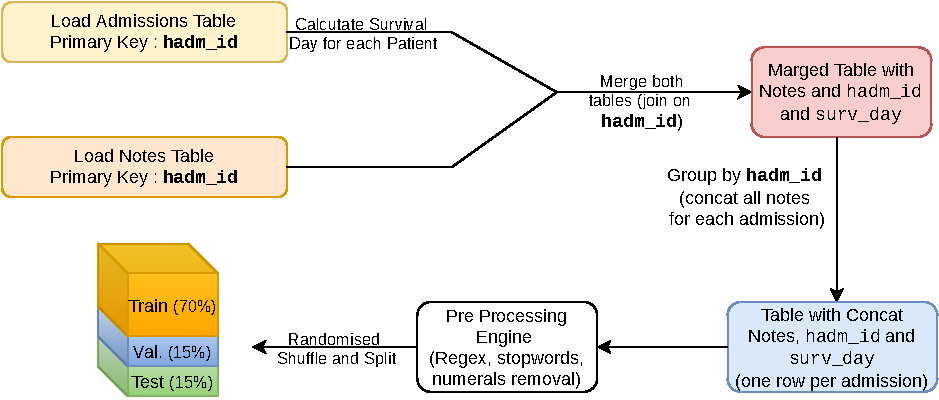
\includegraphics[width=0.7\linewidth]{hca-flow}
	\caption{Workflow of data preparation}
	\label{fig:hca-flow}
\end{figure}



\section{Model Description \& Motive}\label{model}
Although recent work by \citet{rajkomar2018scalable} has achieved  0.94 AUROC for in-hospital mortality; however, they have used sophisticated deep learning techniques. As already explained earlier in motivation, we are keen on building simple as well as an interpretable model for mortality prediction. Hence, we will use simple models such as Logistic Regression, Trees, and Support Vector Machines.

Since we are using bag of words approach with logistic regression for model building we can plot the most important features for each \textbf{True} and \textbf{False} survival class.
This approach helped us in finding out few more stop words that our model is learning which are any-ways redundant. 

\textbf{True} = [\texttt{ml, should, time, it, been, cm, cc, dr}]

\textbf{False} = [\texttt{po, off, c, i, level, to, s, at}]

We added them in our new stop words list subsequently removing them from our vocabulary.  We experimented with various hyper-parameters for all models using standard methodology and used ones, which provided best performance. These curves are shown in Figure \ref{learning}.
We also plotted the learning curves to find out that addition of more data is not likely to improve the performance of our simple model.  


\begin{figure}[h!]
	\centering
	\begin{subfigure}[b]{0.475\textwidth}
		\centering
		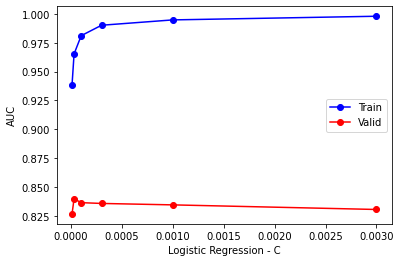
\includegraphics[width=\textwidth]{prm1}
		\caption[Network2]%
		{{\small C Value}}    

	\end{subfigure}
	\hfill
	\begin{subfigure}[b]{0.475\textwidth}  
		\centering 
		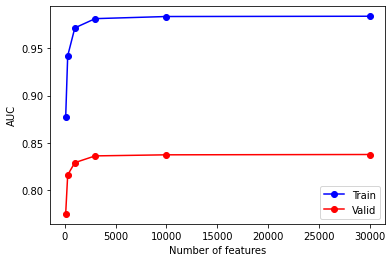
\includegraphics[width=\textwidth]{prm2}
		\caption[]%
		{{\small Number of Features}}    
	\end{subfigure}
\caption{Choice of Hyperparamter for logistic regression}
\label{learning}
\end{figure}

\paragraph{Sentiment Analysis} Following the idea of \citet{Smith18}, we tried to see whether our concatenated notes have any sentiment which can be used as a proxy for mortality. Since sentiment analysis is inherently a supervised learning problem but as we don't have any labelled data of true sentiments we have resorted to using syntactic approach and used Textblob NLP Library. Using \texttt{v0.16.0} of this library we extracted two syntactic features from the text -- polarity and subjectivity.
The Textblob algorithm tokenizes the text, performs POS tagging, and uses a lexicon to give a sentiment polarity and subjectivity score. 
We used these features with SAPSII score (which are already provided in MIMIC dataset) to do the survival analysis of the patients. We partitioned the polarity and subjectivity into 4 quartiles and plotted the Kaplan Meier curve \cite{kaplan1958nonparametric}. The survival analysis was performed in  R (v 3.6.3) using \texttt{survminer}.
First for a preliminary analysis only subjectivity (as obtained from nursing notes -- one of the dimension of sentiment) was used to plot the survival curve with $p<0.0001$. The results are shown in Figure \ref{fig:surv1}.
\begin{figure}[h!]
	\centering
	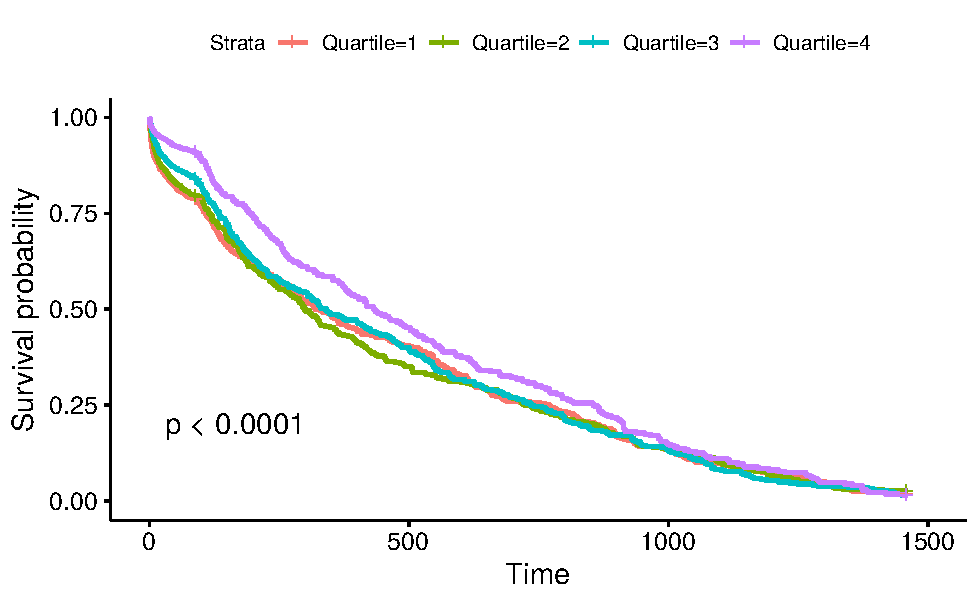
\includegraphics[width=0.7\linewidth]{surv1}
	\caption{Survival Curves using Only Subjectivity and SAPSII Score}
	\label{fig:surv1}
\end{figure}
The results for Kaplan Meier curve (plotted using both subjectivity, polarity and SAPSII score) is reproduced in Figure \ref{fig:km}.   
\section{Results and Analysis}\label{evaluation}
This section assess the performance of our model. Specifically in next subsection \ref{metric} we define the evaluation metric and subsequent subsection \ref{res} reports the results. 
\subsection{Evaluation Metrics}\label{metric}

\begin{itemize}
	\item We have used Area under the receiver operator curve (\textbf{AUC}) to judge the performance of the model. This metric is consistent with  other studies published in the domain \cite{DudaHart2nd}. \item Apart from AUC, we reported \textbf{Accuracy} as well. Accuracy is defined as $\displaystyle \frac{\sum \textrm{TP} + \sum \textrm{TN}}{\sum \textrm{Total~Population}}$. \item We also reported \textbf{Specificity}, which is defined as $${\displaystyle {{\frac {\textrm{number of true negatives}}{{\textrm{number of true negatives}}+{\textrm{number of false positives}}}}}}$$
\end{itemize}
\subsection{Results}\label{res}




\begin{table}[h!]
	\label{table:res1}
	\centering
	\resizebox{0.85\textwidth}{!}{%
		\begin{tabular}{@{}lccc|ccc@{}}
			\toprule
			Model $\rightarrow$  & \multicolumn{3}{c}{\cellcolor[HTML]{B2B2B2}Logistic Regression} & \multicolumn{3}{c}{\cellcolor[HTML]{B2B2B2}Decision Tree} \\ \midrule
			Metric $\rightarrow$ & AUC                    & Accuracy         & Specificity         & AUC            & Accuracy          & Specificity          \\
			7 day Mortality        & 0.891                  & 0.766            & 0.762               & 0.743          & 0.765             & 0.767                \\
			30 day Mortality       & 0.884                  & 0.855            & 0.862               & 0.809          & 0.810             & 0.811                \\
			6 month Mortality      & 0.641                  & 0.599            & 0.597               & 0.554          & 0.662             & 0.671                \\
			1 year Mortality       & \textbf{0.607}         & 0.569            & 0.567               & 0.550          & 0.542             & 0.540                \\
			& \textbf{}              &                  &                     &                &                   &                      \\\hline
			Model $\rightarrow$  & \multicolumn{3}{c}{\cellcolor[HTML]{B2B2B2}XG Boost}            & \multicolumn{3}{c}{\cellcolor[HTML]{B2B2B2}SVM}           \\\hline
			Metric $\rightarrow$ & AUC                    & Accuracy         & Specificity         & AUC            & Accuracy          & Specificity          \\
			7 day Mortality        & \textbf{0.899}         & 0.834            & 0.834               & 0.739          & 0.679             & 0.68                 \\
			30 day Mortality       & \textbf{0.926}         & 0.906            & 0.915               & 0.665          & 0.705             & 0.744                \\
			6 month Mortality      & \textbf{0.678}         & 0.640            & 0.640               & 0.569          & 0.600             & 0.609                \\
			1 year Mortality       & 0.604                  & 0.597            & 0.602               & 0.500          & 0.515             & 0.536                \\ \bottomrule
		\end{tabular}%
	}
	\caption{Evaluation Metric for Various Models}
\label{tab1}
\end{table}


Results from our experiment are presented in Table \ref{tab1}.
Among all the models experimented Logistic Regression and XG Boost performed better compared to others. 
The best AUC was achieved for 30 day mortality prediction and performance drops as we aim for 6 month or 1 year long mortality prediction. The AUC plots for various survival class using simple Logistic Regression model is shown is Figure \ref{fig:lr}. 


\begin{figure*}[h!]
	\centering
	\begin{subfigure}[b]{0.475\textwidth}
		\centering
		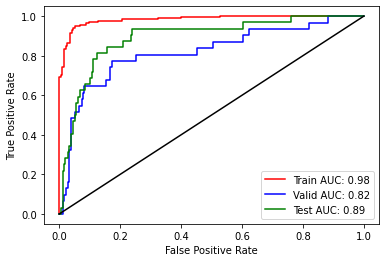
\includegraphics[width=\textwidth]{7d}
		\caption[Network2]%
		{{\small 7 day mortality}}    
		\label{fig:mean and std of net14}
	\end{subfigure}
	\hfill
	\begin{subfigure}[b]{0.475\textwidth}  
		\centering 
		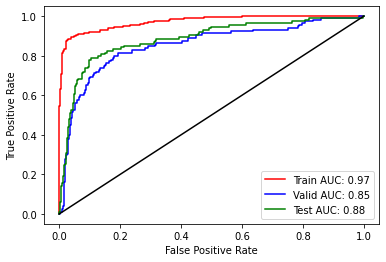
\includegraphics[width=\textwidth]{30d}
		\caption[]%
		{{\small 30 day mortality}}    
		\label{fig:mean and std of net24}
	\end{subfigure}
	\vskip\baselineskip
	\begin{subfigure}[b]{0.475\textwidth}   
		\centering 
		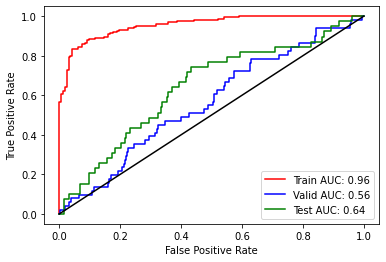
\includegraphics[width=\textwidth]{180d}
		\caption[]%
		{{\small 180 day mortality}}    
		\label{fig:mean and std of net34}
	\end{subfigure}
	\quad
	\begin{subfigure}[b]{0.475\textwidth}   
		\centering 
		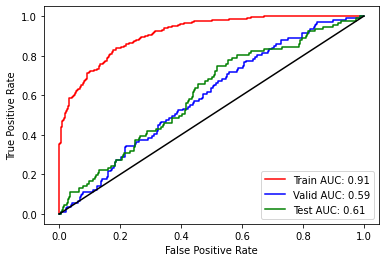
\includegraphics[width=\textwidth]{365d}
		\caption[]%
		{{\small 365 day mortality}}    
		\label{fig:mean and std of net44}
	\end{subfigure}
	\caption[ The average and standard deviation of critical parameters ]
	{\small AUC Curve for 7/30/180/365 day mortality} 
	\label{fig:lr}
\end{figure*}

 We hypothesize that nursing notes have opinions and other latent features which are predictive of near mortality viz. one week or one month. But as we try to predict the longer period mortality such as six month or one year  it becomes increasingly difficult. 

We have plotted the KM curve (in Figure \ref{fig:km}) which has  
polarity and subjectivity quartiles somewhat separated. Top two quartiles are well separated but bottom two have some overlap. \citet{Smith18} in their work have statistically shown that quartiles are nicely separated. In our work may be concatenating the notes and taking all the notes including (discharge notes too) might be a reason for overlap, it needs statistical investigation. 

\begin{figure}[h!]
	\centering
	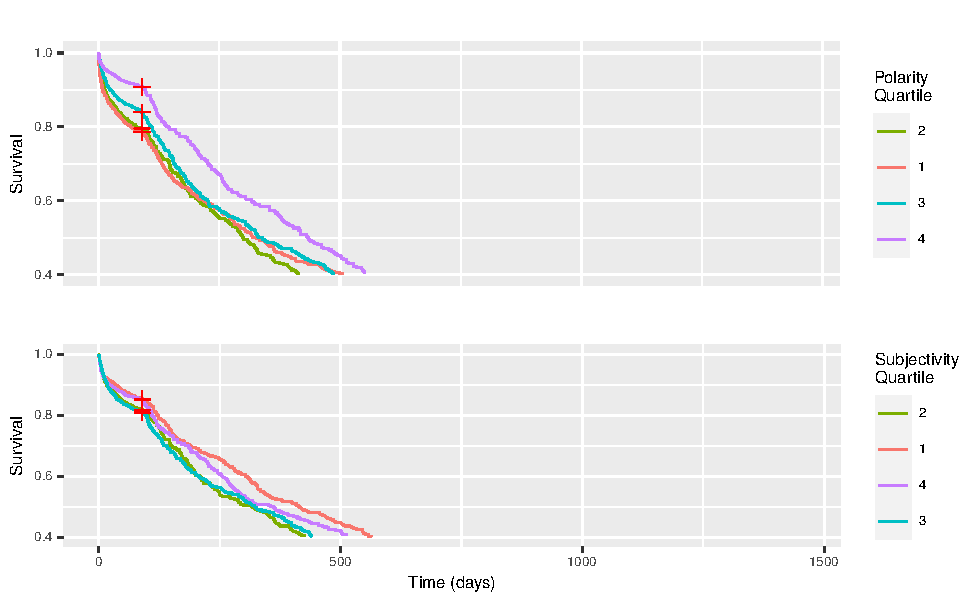
\includegraphics[width=\linewidth]{km.pdf}
	\caption{Kaplan Meier Curve}
	\label{fig:km}
\end{figure}
\section{Discussion \& Future Directions}
While our model does not beat the state
 of the art models for mortality prediction from clinical notes; however,
it compares favourably with most given its simplicity. It clearly shows that unstructured text in the EHR notes contains meaningful information that can be mined for building intelligent medical decision support systems.
Our data is from a single hospital, so patients have somewhat similar demography as well as nurse, and physicians are the same; their way of recording the opinion is somewhat similar. If we could use the data from multiple sources, we can genuinely validate our claim.


We plan to incorporate other structural data (which is mostly time series such as patient measurements, etc.) in our model; and build a simple multimodal fusion model that can leverage both structural as well as unstructured free form text. The sentiment of the notes can also be incorporated into the model, as already shown above and empirical work by \citet{Smith18} support this too, that sentiment and opinion of nurse/physician have mortality prediction property. On these lines, we can improve our model’s utility.

Prediction of mortality remains a complex problem, however by incorporating more information extracted from unstructured data, like nursing notes it might improve the overall performance. 

\section*{Software and Data}

Code is available in github \url{https://github.com/vntkumar8/clinical-notes-mining}. \\
The data is available publicly (to be downloaded) from physionet website \url{https://physionet.org/content/mimiciii/1.4/}.  Due to confidentiality agreement signed between dataset provider, we can not share the data. 

	\bibliography{example}
	
\end{document}
		
